\chapter{\label{ch:solubility}Vibrational Effects in Graphene Nanoribbons}

\minitoc

\section{Introduction}\label{solubility:sec:intro}

As we saw in the last chapter, \glspl{MGNR} could provide a platform to electrically manipulate electronic states at high temperatures. Since spin coherence times up to \si{\micro\second} have been measured in a comparable temperature range~\cite{slota2018magnetic,lombardi2019quantum}, circumstances appear to be ideal for using single \glspl{MGNR} to exploit spin and topological phenomena for quantum applications; however, only devices with sharp features, where all the quantum states can be accessed properly, can be used for quantum experiments.

Because of the strong $\pi-\pi$ interactions between their large conjugated sp$^2$-carbon planes, \glspl{MGNR} can easily aggregate in the solid state and in solution, making the integration of \glspl{MGNR} into electronic nanodevices challenging. For improving liquid-phase \gls{MGNR} dispersion, both physical techniques (i.e., sonication exfoliation~\cite{wang2008room}) and chemical treatment with a strong acid~\cite{shekhirev2017interfacial} have been used. These approaches, however, have limited dispersion effects and, often, \glspl{MGNR} clusters persist.

To date, two basic techniques for producing liquid-phase-dispersible \glspl{MGNR} have been proposed. The first approach involves the addition of alkyl substituents along the edges. For example, dodecyl-decorated \glspl{MGNR} with lateral widths of \SIrange{0.7}{1.1}{\nano\metre} and lengths of more than \SI{200}{\nano\metre} are often the go to choice~\cite{narita2014synthesis}, but strong sonications are unfortunately still necessary, which may be detrimental to the honeycomb lattice, as carbon nanotubes have indicated in the past~\cite{ham2005explanation, vaisman2006role}.

The other approach involves the addition of bulky 3D groups at the periphery of the \glspl{MGNR}. The dimensions of these substituents are typically greater than the graphite interlayer distance $\simeq\SI{0.34}{\nano\metre}$, hence they should dramatically disrupt the $\pi-\pi$ interactions, and aid the dispersion of individual ribbons in the liquid phase. A little shaking or very mild sonication in common organic solvents such as THF, dichloromethane, and toluene is reported to yield homogeneous dispersions~\cite{huang2018intrinsic}.

In this chapter, we will attempt to demonstrate that attaching 3D substituents with a high degree of steric hindrance along the ribbon edges can improve the solubility of graphene nanoribbons in common apolar solvents.

\section{Coulomb-blockade Spectroscopy}\label{solubility:sec:transport}

To test the idea that bulky 3D groups increase the degree of \glspl{MGNR} de-bundling in solution, we tested two nanoribbons carrying two different edge functionalisations. The first was decorated with dodecyl alkyl (\gls{MGNR}\textbf{1}), while in the second  maleimide  groups were used (\gls{MGNR}\textbf{2}) (Fig.~\ref{fig:exp:old_gnr_new_gnr}). Furthermore, to investigate possible differences at the device performance level, we connected these ribbons to two device architectures.

The gate is provided by either an n-doped \ce{Si}/\ce{SiO2} backgate wafer ($t_\textrm{ox}\simeq\SI{300}{\nano\metre}$) or a local \ce{Pd} electrode etched into undoped \ce{Si} and covered by \ce{HfO2} ($t_\textrm{ox}\simeq\SI{10}{\nano\metre}$) (Fig.~\ref{fig:exp:old_gnr_new_gnr}a,b). As mentioned in Ch.\ref{ch:fabrication}, \glspl{MGNR} are added by drop casting from solutions, with a yield of about 5 devices out of 100 electroburned gaps, and the existence of a nanoribbon connecting the two leads is identified as a sharp increase of the conductance $G=\partial I_{\mathrm{SD}} / \partial V_{\mathrm{SD}}$ from $G<\SI{1}{\nano\siemens}$ to $\simeq \SI{100}{\nano\siemens}$.

\begin{figure}[hbtp]
    \begin{center}
        \includegraphics[width=\textwidth]{chapter_solubility/figures/old_gnr_new_gnr.png}
        \caption[Enhancement of Quantum Transport Features by using Bulky Groups]{
            \textbf{a,} The device geometries utilised are illustrated in the diagram: an MGNR (side groups are not shown for clarity) bridges two graphene leads coupled to Au pads. The gate is either an n-doped Si wafer with a 300 nm \ce{SiO2} insulating layer on top or a Pd electrode buried in undoped Si with a $\simeq\SI{10}{\nano\metre}$-thick \ce{HfO2} layer on top (bottom).
            \textbf{b,} False-color scanning electron microscopy images of two typical devices for the two geometries.
            \textbf{c,} The source--drain current against bias and gate voltages are shown in stability diagrams for three devices derived with \gls{GNR}1.
            \textbf{d,} Stability diagrams for three \gls{GNR}2 devices, displaying the source--drain conductance in units of the conductance quantum $G_0$. All measurements are done below $T=\SI{500}{\milli\kelvin}$, and diamonds are labelled with regard to an arbitrary number of electrons, $N$, whenever possible.
        }
        \label{fig:exp:old_gnr_new_gnr}
    \end{center}
\end{figure}
%
According to the operating mechanism of \glspl{SET} outlined in Ch.~\ref{ch:theory}, electrons tunnel through a single channel, whose potential is regulated by $V_\textrm{G}$ whose role is to align the \gls{MGNR} levels in resonance with the leads. Because of Coulomb repulsion, an electron already present in the conduction channel would prevent the flow of additional electrons, thus suppressing the device conductance.

The high degree of bundling expected for \gls{MGNR}\textbf{1} made it impossible to produce \glspl{SET} with only one ribbon bridging the nanogap, and the typical stability diagram shows a large region of suppressed conductance (Fig.~\ref{fig:exp:old_gnr_new_gnr}c), corresponding to the bandgap of semiconducting \glspl{MGNR}, followed by multiple overlapping Coulomb diamonds of varying sizes. From the height of the diamonds, and knowing the ribbon width and length~\cite{shylau2009capacitance}, some of the most discernible diamonds yield $l_\textrm{MGNR} \simeq$ 28, 90, 40, 17, 108, 60, 50, and \SI{38}{\nano\metre}, and no sharp features inside the diamonds could be distinguished.

In contrast, \glspl{SET} produced with \gls{MGNR}\textbf{2} exhibit very clean conduction characteristics and a level of detail equivalent to ultra-clean CNTs (Fig.~\ref{fig:exp:old_gnr_new_gnr}d). The diamonds are distinctly periodic, have identical slopes and diameters, and well-defined edges, indicating that each device has a single nanoribbon. Parallel to the Coulomb edges, the excited states are observable as intense, conductance lines running parallel to the diamonds. The high contact-impedances observed are likely influenced by contact lengths limited by the MGNR length~\cite{grosse2011nanoscale}, which is less than the transfer length.

A zoom-in to one of the diamonds highlights the exceptional cleanliness of the features and a full spectroscopy of the conducting element: the edges of the diamonds are suppressed, and a series of multiple excited states can be clearly observed (Fig.~\ref{fig:exp:sd_fc_fit_lorezFit}a), with a $\hbar\omega_\nu=\SI[separate-uncertainty = true]{7.5(0.1)}{\milli\electronvolt}$ feature common to all devices. We observed a gradual quenching of the edge-conductance suppression upon increasing $T$ (Fig.~\ref{fig:exp:sd_fc_fit_lorezFit}d). Similar to the Franck--Condon principle in molecular spectroscopy, electron--vibron coupling might suppress transport for low-lying vibronic states, because electrons are preferably transmitted when the nuclei-position shifts are minimal.

\section{Analysis of the Franck--Condon Conductance Blockade}\label{solubility:sec:fc}

We shall now attempt to explain the suppression of conductance lines parallel to diamond edges within the Franck--Condon blockade framework.


\begin{figure}[hbtp]
    \begin{center}
        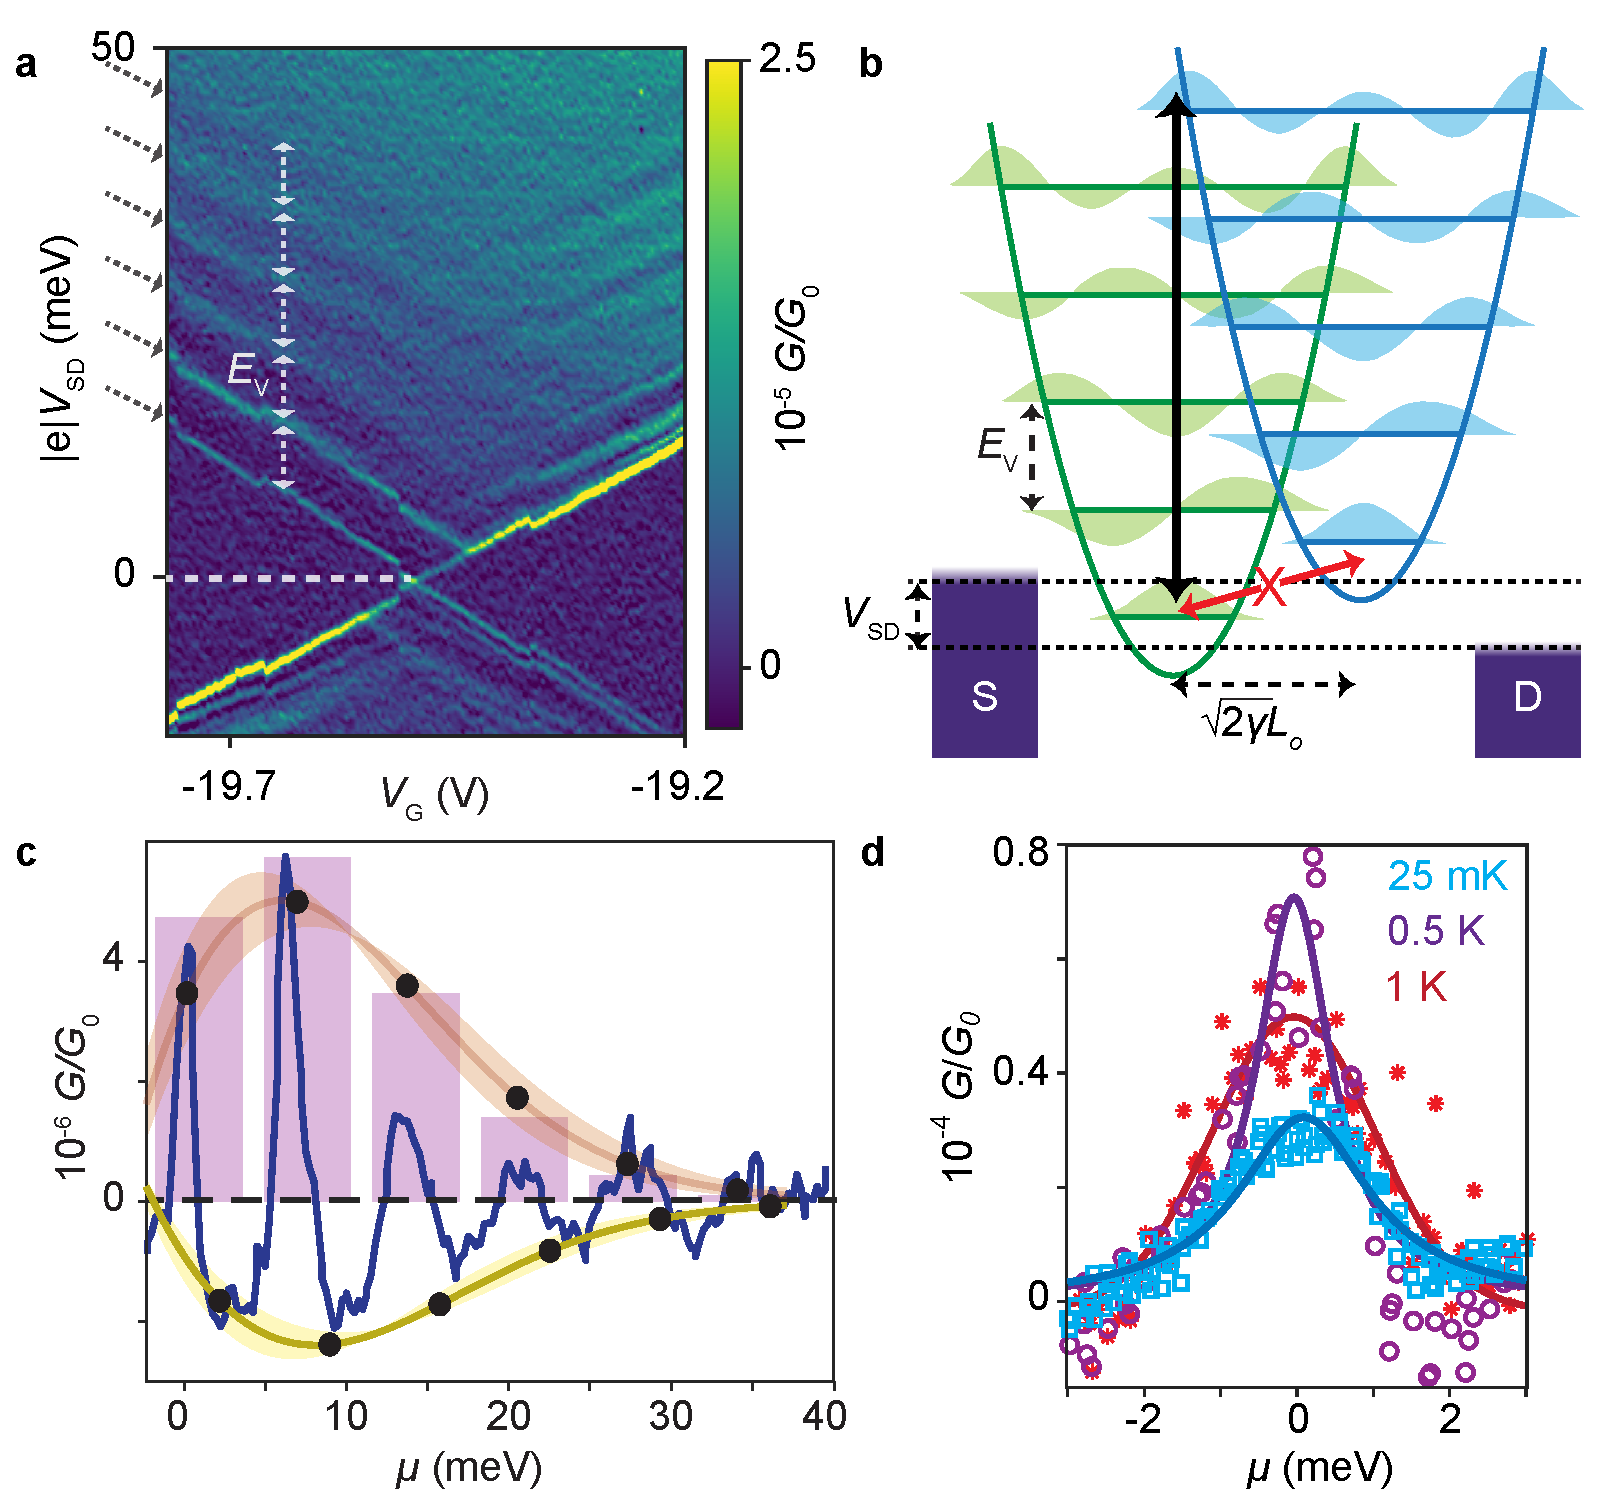
\includegraphics[width=\textwidth]{chapter_solubility/figures/sd_fc_fit_lorezFit.pdf}
        \caption[Franck--Condon Bloackade in MGNR]{
            \textbf{a,} Detail of vibrational state suppression in the differential conductance $G$, in units of quantum conductance $G_0$ versus $V_\textrm{SD}$ and $V_\textrm{G}$. Arrows indicate the excited states, which we assign to vibrational given the equal spacing between them. $T=\SI{20}{\milli\kelvin}$.
            \textbf{b,} The Frank--Condon blockade in the transport properties of nanodevices is depicted schematically, with the equilibrium coordinates for two adjacent charge states (green and blue) represented horizontally. Strong vibronic coupling suppresses ground-to-ground transitions exponentially, whereas ground-to-excited-state transitions become viable at higher bias.
            \textbf{c,} Blockade peaks as a function of the chemical potential $\mu$ as experimentally observed (blue line) and as expected by Frank--Condon theory for maxima (orange) and minima (yellow). Poisson histogram for the vibrational quanta (puple) is superimposed.
            \textbf{d,} Lifting of the Frank--Condon blockade for a transmission channel upon increasing the temperature from \SI{25}{\milli\kelvin} (blue) to \SI{1}{\kelvin} (red), together with Lorentzian fits to the data (solid lines).
        }
        \label{fig:exp:sd_fc_fit_lorezFit}
    \end{center}
\end{figure}

According to standard electronic absorption theory, the spectrum resulting from the excitation with wavelenths within the vibrational region is a progression of absorption peaks rising separated by multiples of the vibrational quanta, and with the intensity lines of the spectrum that follows a Poisson distribution~\cite{karabunarliev2000rigorous}. The amplitude of each peak in the vibrational progression is governed by the Franck--Condon factors, which are defined as transition probabilities, according to standard quantum theory, between the vibrational states of two different electronic states (ground and excited states) over many vibrational modes.

If we assign the excitation of vibrational states to the equispaced parallel conductance lines within a Coulomb cone, we might be able to link the Franck--Condon factor to the \gls{DC} conductance maxima. Thus, by extracting and averaging within a  bias window parallel lines to the Coulomb edges, we observed that the conductance peaks follows a known progression~\cite{leturcq2009franck}.

Franck--Condon theory describes the coupling electron--vibron $\gamma$, i.e. how an addition of an electron changes the electronic wave function and produces a shift in the equilibrium coordinate of a molecule. If $\gamma$ is large, then charge transport may be suppressed through low-lying vibronic MGNR states (Fig.~\ref{fig:exp:sd_fc_fit_lorezFit}b). Furthermore, Franck--Condon theory predicts that the peak conductance of the vibronic transitions, $G_n^{\max }$, follows a Poisson distribution in terms of the vibron quantum number $n$,

\begin{equation}\label{eq:franck_condon_fit}
    G_n^{\max }=\frac{\gamma^n}{n !} e^{-\gamma},
\end{equation}
%    
By fitting the averaged conductance trace within a Coulomb cone with Eq.~\ref{eq:franck_condon_fit} we extract an electron--vibron coupling $\gamma=1.5 \pm 0.2$. Fig.~\ref{fig:exp:sd_fc_fit_lorezFit}c shows the progression of the vibronic peaks, which arise when an electron tunnels through a molecular orbital and simultaneously excites a molecular vibrations~\cite{van2013suppression}.

A hint of Franck-Condon suppression apparent from Figure Fig.~\ref{fig:exp:sd_fc_fit_lorezFit}d where an increase in $T$ from \SI{25}{\milli\kelvin} to \SI{0.5}{\kelvin} is followed by an increase in $G$. A further increase to \SI{1}{\kelvin} decreases $G$ due to significant temperature broadening. The same figure was used to calculate the electrode--\gls{MGNR} coupling energy $\Gamma\simeq\SI[separate-uncertainty = true]{185(30)}{\micro\electronvolt}$, in line with the estimate detailed in the previous chapter.



\section{Simulation of the Stability Diagram}\label{solubility:sec:simulation}

We shall now try to validate our conclusions exposed in the previous section about the possibility of having a Franck--Condon suppression of the conductance by reproducing the experimental observation with a simulated model. We shall use, to this end, the model exposed in Sec.~\ref{ch:theory:sec:vibrations}, and assume that the molecular energy level, $\mu=C_\textrm{S} V_\textrm{SD}-C_\textrm{G} V_\textrm{G}$, shifts with both bias and gate voltages.

\begin{figure}[hbtp]
    \begin{center}
        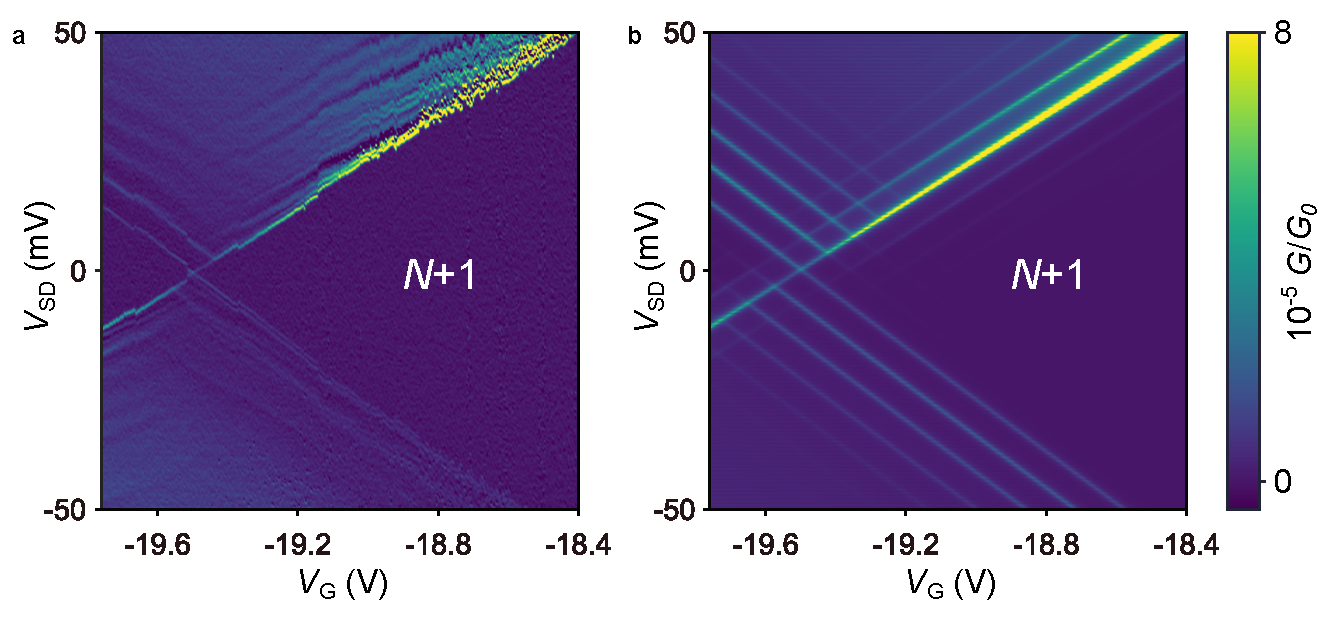
\includegraphics[width=\textwidth]{chapter_solubility/figures/sd_experimental_simulated.pdf}
        \caption[Single-Mode and Phonon Bath Models for MGNR Vibrations]
        {
            Maps of the conductance for the same transition as in Fig.~\ref{fig:exp:sd_fc_fit_lorezFit}a, plotted on identical colour scale. \textbf{a,} Experimental conductance map for the same charge transition of Fig.~\ref{fig:exp:sd_fc_fit_lorezFit}a. \textbf{b,} Simulated conductance using Eq.~\ref{eq:initial_vibration_equation}--\ref{eq:final_vibration_equation} and the parameters from Tab.~\ref{tab:simulated_stability_diagram}. Integrals were evaluated using the Simpson's rule as implatemented in Numpy.
        }
        \label{fig:exp:sd_experimental_theory}
    \end{center}
\end{figure}
%
The calculated conductance $G$ (Tab.~\ref{tab:simulated_stability_diagram} reports the simulation parameters) is plotted as a function of $V_\textrm{SD}$ and $V_\textrm{G}$, and is displayed next to an experimental stability diagram in Fig.~\ref{fig:exp:sd_experimental_theory}. The calculated and experimental stability diagrams match each other extremely well. Importantly, the calculated diagram shows that the single-mode--environment model reproduces the main features of our data, i.e. conductance lines equally spaced by $E_v\simeq\SI{7.5}{\milli\electronvolt}$, a significant contribution from the phonon bath and conductance asymmetry with bias. The calculated stability diagram contains additional conductance sidebands in the blocked regions that are not present in the experimental diagram.



\begin{table}
    \caption{\label{tab:simulated_stability_diagram}
        Simulation parameter for the vibrational electron transport model}
    \resizebox{\columnwidth}{!}{%
        \begin{tabular}{ccccccccc}
            \hline $T$           & $\hbar\omega_\textrm{q}$   & $\hbar\omega_\textrm{c}$   & $\hbar g_\textrm{q}$       & $\lambda$                  & $\Gamma_\textrm{S}$        & $\Gamma_\textrm{D}$        & $C_\textrm{S}$      & $C_\textrm{G}$                         \\
            (\si{\milli\kelvin}) & (\si{\milli\electronvolt}) & (\si{\milli\electronvolt}) & (\si{\milli\electronvolt}) & (\si{\milli\electronvolt}) & (\si{\milli\electronvolt}) & (\si{\milli\electronvolt}) & (\si{\femto\farad}) & (\si{\femto\farad})                    \\
            \hline
            25                   & 7                          & 8.5                        & 20                         & 150                        & \SI{1.2e-3}{}              & 0.5                        & 0.54                & \SI{2.25e-2}{}                 \Tsmall \\
            \hline
        \end{tabular}%
    }
\end{table}


We explain the increase of background conductance at high bias as the result of the coupling with an increasing number of phonon modes in the bath. This hypothesis would also explain the different tunneling rates we had to use to reproduce the spectrum, which are the reason for the observed $V_\textrm{SD}$ asymmetry, and may be caused by larger contact length $L_\textrm{c}$ between the \gls{MGNR} and the drain than the source lead. The model does not take into account the slanted conductance lines originating from the leads and does therefore not reproduce these.



\section{Role of the Maleimide Groups: \textit{Ab-Initio} and Statistical Analysis}

Since our \glspl{MGNR} are synthesised with molecular precision through bottom-up synthesis, we deem appropriate to calculate from \textit{ab-initio} the vibrational properties of a simplified \gls{MGNR} structure and to attempt elucidating the origin of the Franck--Condon blockade and the nature of the vibrational mode we identified through the conductance measurements.

DFT calculations were performed using the GGA--PBE functional as implemented in the Siesta package~\cite{soler2002siesta,garcia2020siesta}. One structure was calculated with edges terminated by hydrogen atoms, another with anthracene groups, and the third with maleimide  groups (Fig.~\ref{fig:exp:phonon_mode_comparison} and Fig.~\ref{fig:exp:phonon_anthracene_maleimide }). Along the non-periodic directions an adequate number of vacuum states were added in order to avoid unwanted interactions. An energy cut-off of \SI{400}{\unit{Ry}} was used together with a $20\times 1\times 1$ Monkhorst--Pack grid constructed along the three Cartesian directions. The structure was optimized until the maximum force on the atoms was less than \SI{0.01}{\electronvolt\per\angstrom}. The dispersion relation is calculated with a supercell size of $3\times 1\times 1$, where 3 represents 3 unit cells along the periodic direction, and atomic displacements of the $\Gamma$ phonon mode are visualised with the software XCrySDen. The phonon disperions were calculated using the same numerical constraints.

\begin{figure}[hbtp]
    \begin{center}
        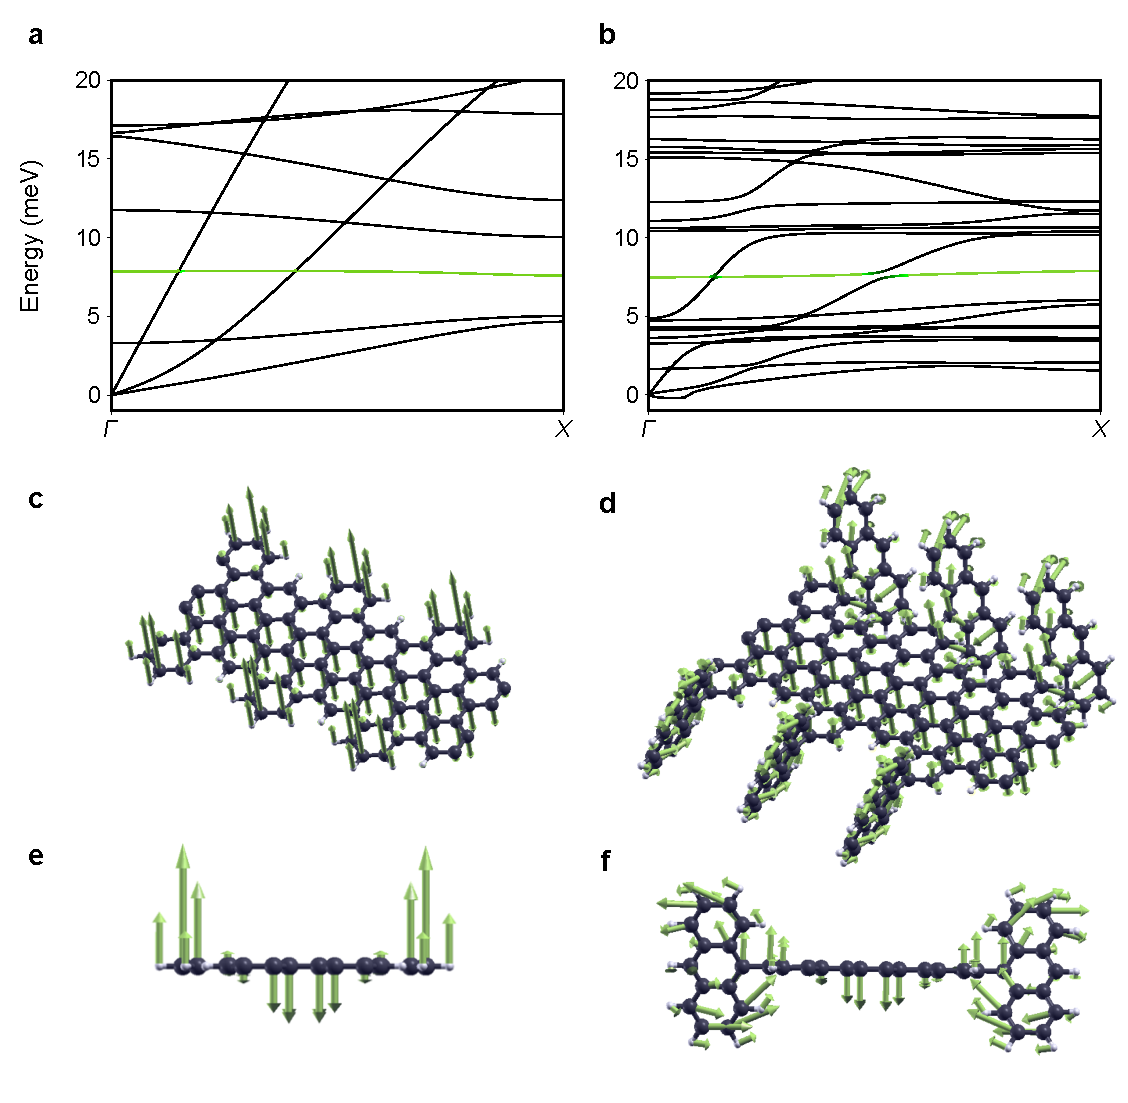
\includegraphics[width=\textwidth]{chapter_solubility/figures/Phonon_Mode_Comparison.pdf}
        \caption[Phonon Dispersion MGNR: The Role of Anthracene Groups]{
            \textbf{a,}
            \textbf{b,} Energy dispersion of the lowest vibrational modes when anthracene groups are attached to the edges, with the one at \SI{7.5}{\milli\electronvolt} highlighted in green.
            \textbf{c,}
            \textbf{d,} Relative displacement of the atoms for the \SI{7.5}{\milli\electronvolt} vibrational mode at $\Gamma$ point.
            \textbf{e,}
            \textbf{f,} Side view of the relative displacement for the \SI{7.5}{\milli\electronvolt} vibrational mode at $\Gamma$ point.
        }
        \label{fig:exp:phonon_mode_comparison}
    \end{center}
\end{figure}


\begin{figure}[hbtp]
    \begin{center}
        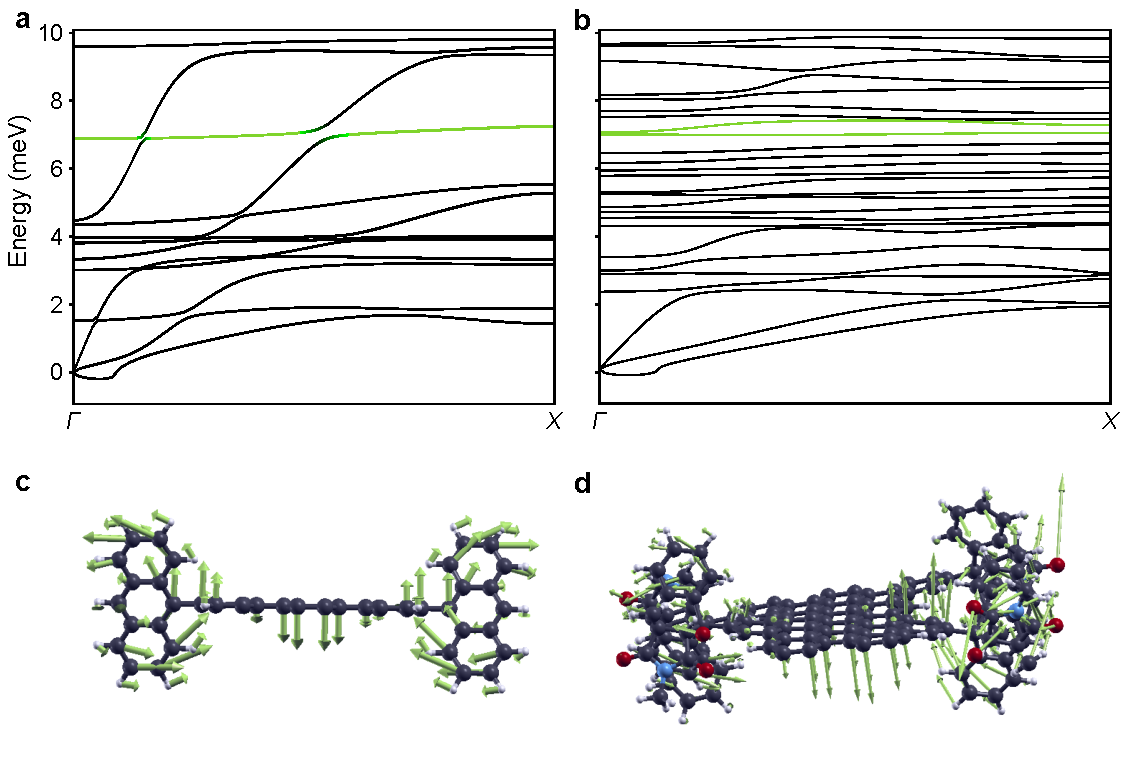
\includegraphics[width=\textwidth]{chapter_solubility/figures/phonon_anthracene_malimide.pdf}
        \caption[Phonon Dispersion MGNR: The Role of Maleimide Groups]
        {
            \textbf{a,}
            \textbf{b,} Energy dispersion of the lowest vibrational modes when maleimide  groups are attached to the edges, with the one at \SI{7.5}{\milli\electronvolt} highlighted in green.
            \textbf{c,}
            \textbf{d,} Side view of the relative displacement of the atoms for the \SI{7.5}{\milli\electronvolt} vibrational mode at $\Gamma$ point.
        }
        \label{fig:exp:phonon_anthracene_maleimide }
    \end{center}
\end{figure}

\begin{figure}[hbtp]
    \begin{center}
        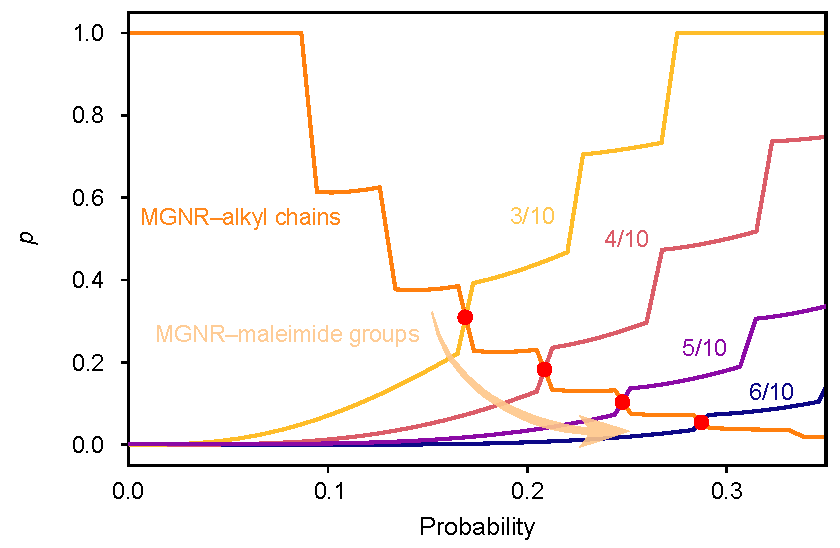
\includegraphics[width=\textwidth]{chapter_solubility/figures/p_test.pdf}
        \caption[MGNR--Maleimide Statistics: A p-Value Argument]{
            $p$-value as a function of the likelihood of obtaining a \gls{SET} (probability, for short) when using \gls{MGNR}\textbf{2}. The numerical figures represent the number of observed \glspl{SET} relative to the overall number of devices cooled down in the fridge. The $p$-value decreases by more than an order of magnitude as the number of observed \glspl{SET} increases by 2 units.
        }
        \label{fig:exp:p_test}
    \end{center}
\end{figure}

Firstly, we calculated the effect the anthracene groups have on the atom displacements compared to the base case (Fig.~\ref{fig:exp:phonon_mode_comparison}). We can qualitatively assess the emergence of new phonon modes, the majority of which are exclusive to the anthracene groups, and a few of which correlate to the \gls{MGNR} backbone. In addition, the three acoustic phonons combine with optical phonons, resulting in the constant dispersion of new hybrid phonons throughout the Brillouin zone. Particularly, the dispersion relation reveals that the phonon mode at  $\hbar\omega_\nu=\SI{7.50}{\milli\electronvolt}$ is robust at the $\Gamma$ point and experiences mode mixing at certain wavevectors.

In addition, at the $\Gamma$ point one mode is reduced from \SI{7.86}{\milli\electronvolt} to \SI{7.48}{\milli\electronvolt}, matching the experimental value (Sec.~\ref{solubility:sec:fc}) much more accurately. We conclude, using the visualisation tool, that this phonon mode may be responsible for the MGNR backbone bending as well as the quenching of the amplitude oscillation of the atoms along the edges.

Secondly, we looked at how the inclusion of maleimide  groups on the phonon dispersion following the introduction of the maleimide  groups (Fig.~\ref{fig:exp:phonon_anthracene_maleimide }). Compared to the anthracene, the acoustic mode at $\hbar\omega = \SI{7.48}{\milli\electronvolt}$ induce a stronger ribbon backbone bending (Fig.~\ref{fig:exp:phonon_anthracene_maleimide }d), as also put in evidence by the greater mode amplitude. Furthermore, we note that the displacement of core-backbone atoms remains approximately constant, whereas cove-edge atoms become more rigid. This qualitative observation seems to suggest that bending will be primarily confined to the backbone centre when 3D side groups are introduced.

\co{SET formation probability argument}
Despite being rigorous, our analysis may be incomplete. In fact, while \gls{DFT} is commonly regarded as the \textit{de facto} standard for calculating molecular and physical properties in a reasonable amount of time, issues sometime arise when accurate estimates are required. Because our system includes not only the ribbon but also the graphene leads, the question of whether maleimide groups promotes or not the dispersability of \glspl{MGNR} in a solvent, thus boosting the chances to have ultra-clean \glspl{SET} may still arise. In order to answer this question, we will use a simple yet powerful idea from standard statistics.

In order to exclude the possibility that the observed number of \glspl{SET} (Fig.~\ref{fig:exp:old_gnr_new_gnr}) are produced merely by chance, we shall use statistics to test if out of the total number of devices the \gls{SET} formation probabilities when either \gls{MGNR}\textbf{1} or \gls{MGNR}\textbf{2} are employed are generated from the same statistical process (null hypothesis, $H_0$). By setting the $p$-value threshold at the common value $p=0.05$ means that we have a 5\% chance of falsely concluding that 3D bulky groups do not promote the formation of ultra-clean \glspl{SET}, meaning that the \gls{SET} formation probability are generated by the same statistical process.

We made one chip by depositing \gls{MGNR}\textbf{1} on top of \glspl{GTJ} and three by dropcasting \gls{MGNR}\textbf{2}. We then wirebonded 10 devices on each chip and cooled them down at \SI{25}{\milli\kelvin}. We counted the number of \glspl{SET} for each chip by measuring high-resolution full-range stability maps and selecting whether or not to include a device based on visual inspection.

Assuming we can pick up a SET with equal chance by dropcasting either \gls{MGNR}\textbf{1} or \gls{MGNR}\textbf{2}, we can run a binomial test to get the $p$-value of obtaining 0/10 \glspl{SET} when \gls{MGNR}\textbf{1} is dropcasted. The results are stored in Tab.~\ref{tab:p_values} and shown in Fig.~\ref{fig:exp:p_test}.

\begin{table}
    \caption{\label{tab:p_values} Statistics of the SET formation probability of all the measured devices.}
    \centering
    \begin{tabular}{ccccc}
        \hline MGNR Type           & \textbf{1} & \textbf{2} & \textbf{2} & \textbf{2}                           \\
        Number of Devices Cooldown & 10         & 10         & 10         & 10                                \T \\
        Number of SETs per chip    & 0/10       & 3/10       & 4/10       & 6/10                                 \\
        $p$ value                  & ---        & 0.307      & 0.182      & 0.056                                \\
        \hline
    \end{tabular}
\end{table}

These results seems to suggest that we cannot exclude at the 95\% confidence level that the SET produced when using the 3D bulky groups are produce by chance. A couple of clarifications are, however, necessary. Firstly, statistical validity of are such only in the case the experiment is repeated in the exact same conditions. Here, however, the number of observed SET across several chips cooled down is given by the total number of devices surviving the thermal shock from going to 50 K down to cryogenic temperature. This in fact does not exclude that more SET could have been actually formed but could not been measured simply due to this secondary process interfering with our statsitics.

These findings appear to imply that, at the 95\% confidence level, we cannot rule out the possibility that the SET obtained when using the 3D bulky groups was produced by chance. However, a number of specifics are required. To begin, statistical validity exists only if the experiment is repeated under same conditions. However, in this case, the number of detected \glspl{SET} across numerous cooled chips is determined by the total number of devices surviving the thermal shock from \SI{50}{\kelvin} to cryogenic temperature. This does not rule out the possibility that more \glspl{SET} were generated but could not be measured due to this secondary process interfering with our statistics.

Secondly, the number of data collected may be not sufficient for an accurate and precise statistical analysis. In particular, small samples (number of data is less than 10) tend to underestimate the standard deviation of the population, as well as having means frequently far from the true mean~\cite{reus2012statistical, reuter2012signatures}. Therefore, at this stage we cannot exclude the role the bulky groups have on obtaining ultra-clean single-electron transistors.

Second, the amount of data collected may be insufficient for a thorough statistical analysis. Small samples (fewer than 10) in particular tend to underestimate the population standard deviation, as well as having means that are frequently distant from the true (population) mean~\cite{reus2012statistical, reuter2012signatures}. As a result, we cannot exclude the hypothesis that maleimide groups are essential to fabricate ultra-clean \glspl{SET}, but also we cannot confirm it from a statistical standpoint at this time. Future study may employ a cryogenic multiplexer to increase the number of devices measurable with a single cooldown by an order of magnitude, expanding the sample size and providing more robust and accurate statistics.

\section{Outlook and Perspectives}\label{solubility:sec:summary}

When compared to $\gamma$ values reported for in-situ generated suspended \glspl{CNT}, our findings are lower for some but higher for others (Tab.~\ref{tab:electron_vibron_couplings}), and suggest enhanced electron--vibron coupling in graphene nanoribbons~\cite{zhou2019electron}.

Remarkably, our values are equivalent to those obtained in molecular junctions comprising \ce{C140}, but far greater than those observed in base \ce{C60}. We can hypothesise that low-energy modes in the substrate phonon bath may facilitate transport near the diamond edges, so suppressing the true magnitude of the Franck--Condon effect. Decoupling the nanoribbon from the substrate environment via suspension should therefore result in higher $\gamma$ values than for nanotubes~\cite{sapmaz2006tunneling}.

\begin{table}
    \caption{\label{tab:electron_vibron_couplings}
        Electron--vibron coupling has been described in the literature for a variety of devices.}
    \begin{center}
        \begin{tabular}{ccc}
            \hline Material               & $\gamma$     & Reference                                          \\
            type                          &              &                                                    \\
            \hline
            \ce{C60}                      & $\ll$ 1      & \cite{park2000nanomechanical}              \Tsmall \\
            CNT                           & 0.5--1.1     & \cite{sapmaz2006tunneling}                         \\
            \ce{C140}                     & $\simeq 1.4$ & \cite{pasupathy2005vibration}                      \\
            MGNR                          & $1.5\pm0.2$  & This work                                          \\
            \ce{C60} (graphene junctions) & 3            & \cite{lau2016redox}                                \\
            CNT                           & 3.3          & \cite{leturcq2009franck}                           \\
            \ce{Fe4} SMM                  & 4.2          & \cite{burzuri2014franck}                           \\
            \hline
        \end{tabular}
    \end{center}
\end{table}

Furthermore, first-principles studies have suggested the existence of edge-localised nonlinear modes in \glspl{AGNR} with energies \SIrange{6.8}{8.7}{\milli\electronvolt}~\cite{savin2016localized}, which would encompass our experimental and \gls{DFT} findings. Based on these, we conclude that the electronic wave function of \gls{GNR} have a large non-zero overlap with the bending mode at $\hbar\omega_\nu\simeq\SI{7.5}{\milli\electronvolt}$, resulting in high electron--vibron coupling which would explain the larger conductance compared to lower-lying vibrons~\cite{droth2011acoustic}.

As we saw in Ch.~\ref{ch:introduction}, the nanotube electronic structure is heavily dependent on the tube chirality, length, and radius, which are difficult to control and may greatly vary across devices. On the other hand, \glspl{MGNR} can now be engineered with molecular accuracy, thus allowing the production of devices with more uniform performance. Currently, one of the biggest challenge is the synthesis of nanoribbons of with length spanning several hundreds of nanometer, which should lead to a higher control when positioned on top of devices.

\section{Summary}
\glspl{MGNR}\textbf{1} were supplied by the group of Akimitsu Narita, whereas \glspl{MGNR}\textbf{2} were synthesised in Dresden by the group of Xinliang Feng. The Franck--Condon analysis was undertaken by Dr Simen Sopp (see also~\cite{sopp2021phd}), whereas I acquired temperature data and conducted the corresponding analysis. Fanmiao Kong was responsible for the phonon calculations. Dr Alex Gee supported me in fabricating the devices when I was compelled to stay out of the lab for more than a month owing to covid-19 infection and subsequent health issues that necessitated medical care.